% Chapter 1

\chapter{Literature Review} % Main chapter title

\label{literaturereview} % For referencing the chapter elsewhere, use \ref{Chapter1} 

\lhead{Chapter \ref{literaturereview}. \emph{Literature Review}} % This is for the header on each page - perhaps a shortened title

%----------------------------------------------------------------------------------------
\section{Behaviour Change Support Technologies}
Research on ubiquitous computing to support behaviour change  has received a significant amount of attention in a myriad of domains such as computer science, human-computer interaction and healthcare. One of the core research areas is how to design incentive systems that are emotionally engaging and  provide timely feedback in order to persuade people to change their behaviours~\citep{nakajima2013designing}. 

One of the early pioneers of formalizing behaviour change technology as an area of research was B.J. Fogg\footnote{http://bjfogg.com/}, who coined the term ``captology'', which is an acronym for \emph{Computers As Persuasive Technologies} (CAPT-ology). This describes the intentional persuasive effects of information technologies~\citep{fogg1999persuasive}. In persuasive systems, persuasion is intentional and usually implemented through persuasive stimuli, hence providing a system with an ability to persuade~\citep{hamari2014persuasive}. Persuasive technologies have applications in domains such as healthcare, education and training, and environmental sustainability.

According to~\cite{langrial2012digital}, the evolution of research on behaviour change technologies through the realms of computing research started with digital interventions in the early 1990s, which were essentially for intervening behaviours in the area of preventive health, implemented through reminders. This was followed by the era of persuasive technologies: systems that had various functionality that were implemented based on theories related to social learning or comparison, for example.~The third era, which is the current one, involves behaviour change support systems (BCSS) which arrived with models and frameworks that provide guidance on how persuasive technologies should be designed and evaluated for effectiveness. The term BCSS is defined by~\cite{Oinas-Kukkonen:foundation} as ``a socio-technical information system with psychological and behavioural outcomes designed to form, alter or reinforce attitudes, behaviours or an act of complying without using coercion or deception''.

Different models (frameworks) to guide the design and evaluation of persuasive technologies have been proposed, as models from information systems such as the \emph{Technology Acceptance Model} (TAM) have limitations with regard to understanding the effectiveness of persuasive technologies~\citep{Oinas-kukkonen:psd}. Persuasive technologies' models tend to provide nuanced features and characteristics that define such systems.~\cite{fogg2009behavior} proposed a behaviour model for persuasive design which asserted that in order for an individual to carry out a targeted behaviour, there are conditions that need to be met: an individual must have (1) sufficient motivation, (2) the ability to carry out the behaviour, and (3) be triggered to carry out the targeted behaviour.~\cite{fogg2009behavior2} also recommended a behaviour grid that could guide a person intending to design a persuasive technology. In this behaviour grid, persuasive strategies are matched to targeted behaviours. 

Fogg's model\citep{fogg2009behavior} was extended by \cite{Oinas-kukkonen:psd} who arrived with a more comprehensive model known as a \emph{Persuasive System Design} (PSD) model, which proposed three initial steps that need to be carried out in the process of designing a persuasive system: (1) analysing the persuasion context (this deals with aspects such as the intent of persuasion and context of use, user and technology), (2) selecting persuasive features to use in the envisaged persuasive technology, and (3) selecting persuasive strategies to be used (this entails choosing to use either a direct or indirect route of persuasion, depending on the level of comprehension of targeted users). The PSD model also outlined 28 design principles divided into the following five categories: (1) \emph{primary task support}, which includes activities such as reduction of complex behaviours into simple tasks, guiding the user through experiences while persuading them along the way, tailoring persuasive information according to factors relevant to a specific user group, personalization of content, and self-monitoring for users to keep track of their progress towards their specified goals; (2) \emph{dialogue support}, catering to the use of praises, rewards, similarity, liking, reminders etc.; (3) \emph{system credibility support}, which caters to the aspects of trustworthiness, expertise, surface credibility, etc.; and (4) \emph{social support}, which involves aspects of social learning, social comparison and competition.

An extension of the PSD model was the \emph{Outcome Change} (O/C) matrix, which one could use when analysing an intent of persuasion~\citep{Oinas-Kukkonen:foundation}. The O/C matrix matches the type of change that needs to be applied with a specific outcome. A change could either be of compliance (C), behaviour (B)  or attitude (A). An expected outcome could be forming, altering or reinforcing any of the aforementioned types of change. The extended PSD model with O/C matrix is called BCSS, as mentioned in the classes of behaviour change systems above. BCSS is considered to be the foundation for studying persuasive systems and is meant to provide a base for analysis, design and evaluation of persuasive technologies.
 
The aforementioned models suggest how one could explicitly design motivational affordances and measure their effect in the context of persuasive technologies. But these models do not say anything about utilization of motivational affordances in the context of intermediated layers of users that may exist before the information reaches the targeted beneficiary. For the sake of a complete discussion about persuasive technologies, the next section highlights how behaviour change technologies have been applied in the health domain.

\section{Behaviour Change Technologies for Health}
Healthcare providers are eagerly seeking innovative solutions that could help in monitoring and improving patients' health~\citep{higgins2016smartphone}. Innovative ways to support health promotion and management are needed to respond to the healthcare crisis that is the result of an unprecedented increase in lifestyle-related chronic diseases~\citep{arsand:mobile}. Healthcare systems do not have sufficient resources to cope with the increasing burden of chronic diseases~\citep{quinn2008welldoc,arsand:mobile}; hence these innovative ways aims to support the advocating of shifting from physician-centred care to patient-centred care~\citep{higgins2016smartphone,korhonen2010personal}.  Literature has demonstrated the dominance of persuasive technologies targeting health behaviour change. For instance, in one recent systematic review of 95 studies that examined the ability of persuasive technologies to persuade, 47\% of the studies targeted domains of health and exercise~\citep{hamari2014persuasive}. The remaining 53\% was shared by several domains such as ecological consumption and/or behaviour (21\%, second highest) and education/learning/economic (11\%). This indicates that health is an important area of concern when it comes to persuasive technologies.

\cite{chatterjee2009healthy} classified three generations  of technological evolution of hardware and software utilized in implementations of behaviour change interventions in health. The first generation started to emerge from the 1960s and was characterized by the prescriptive nature of information flow from physician, healthcare provider, or technology-based system, to a healthcare recipient.~Decades worth of research has demonstrated the ability of phone-based or simple messaging technologies to improve the quality of both healthcare management and clinical outcomes. The second generation was characterized by the descriptive nature of information interaction between an end user and a persuasive technology. Examples of systems in the second generation included interactive websites and personal data assistants (PDAs), which facilitated and automated tracking of basic health parameters through self-reporting diaries/journals and simple context-aware sensors. The third generation extends the second generation by providing body-wearable sensors that support advanced health monitoring, and the use of context-aware computing to determine when to deliver “just in time” messages.  The second generation was dominated by the use of PCs and later cellphones, while the third generation is dominated mostly by cellphones and ubiquitous computing devices. The future generation is expected to be the one that will have ubiquitous computing integrated seamlessly into people's daily lives and it will be supported with data mining techniques~\citep{chatterjee2009healthy}.

The first and second generations' systems have received the most appraisal because of existing randomized clinical trials. Their dominance is proved by the preponderance of publications that report on the use of web-based interventions integrated with SMS text messaging in clinical settings. Findings from various systematic reviews have reported extensively on the use of reminders and feedback through SMS technologies in areas of diabetes self-management, smoking cessation and weight reduction therapy~\citep{cole2010text,fjeldsoe2009behavior,krishna2009healthcare}. However, there is an indication of mixed results for the effectiveness of cellphone or other ICT interventions for weight loss, with some studies showing positive results while others show negative results. For instance, one randomized controlled trial (RCT) that was carried out for a period of two years~\citep{svetkey2015cell} found that two intervention groups (one using only a smartphone app, and the other using a combination of both a human coach and a smartphone app) did not demonstrate a more significant improvement in weight loss than a control group which was supplied with only pamphlet materials. In addition to mixed findings that are prevalent in such clinical trials, systematic reviews~\citep{cole2010text,kaplan2006can} have also pointed out drawbacks in delivery of such interventions, of including an inability to scale well to specific demographics within resource-constrained contexts, i.e.~in contexts where technology and textual literacies, or sharing of technology among multiple consumers, may become a barrier to effective delivery of such health interventions. From the perspectives of persuasive technology literature, it has also been observed that there is a gap between research in persuasive technologies and RCTs in public health settings.~Literature from the public health domain is has been criticized for tending to lack adequate information on how individual systems are designed. Such systems are usually poorly described, as most work is published by public health practitioners without the involvement of computer scientists~\citep{Oinas-Kukkonen:foundation}. Therefore, it is arduous to interrogate what system attributes contribute to the success or failure of such interventions. 

Persuasive technologies provide the means to personalize health information. Personalization of health information has been advocated within the public health domain as it allows consideration of the individual needs of a person, and it also gives the targeted person a  sense of control over their healthcare~\citep{mccallum2012gamification}. The broad focus of this research was on  personalized technologies that support both  data collection and feedback for the objective of health persuasion. These systems are referred to as wellness applications or personal health informatics. Personal informatics systems have been defined as group tools to support individuals in having self-awareness of various facets of their lives by providing technological means to support the collection and analysis of personal data related to habits, behaviours and thoughts~\citep{li2011personal,li2012personal}. Utilization of personal health informatics in behaviour change is discussed on the next section. 
\section{Personal Informatics for Health Behaviour Change}
A personal informatics system is effective for self-tracking a behaviour because it augments the activity of \emph{self-reflection} by complementing individuals in storing personal events intertwined with context, where such fine details of events are unlikely to be recalled due to limitations in humans' memory~\citep{li2010stage}. A personal informatics system is capable of storing granular information about events, something that is harder for humans to do. The goal of personal informatics systems is to support individuals in having a better understanding of their lifestyle or behaviours. These systems are important for the promotion of positive behaviours in a myriad of domains such as healthy lifestyle~\citep{korhonen2010personal}, recycling~\citep{comber2013designing} and energy conservation~\citep{seligman1977feedback}. 

Research on personal informatics systems tends to focus on effective ways of collecting users' personal data in an effortless manner, and supporting self-reflection through feedback mechanisms~\citep{li2011understanding}. Data collection is usually supported with context-aware sensors and self-reporting mechanisms. Sensors may be coupled with a computing device for both analysis and feedback, or with an external device that transfers data through either wireless means or data cables to a computing device responsible for analysis and feedback.~\cite{nakajima2013designing} proposed the use of a metaphor, \emph{ambient persuasive mirrors}, to describe displays that could support self-reflection of one's own behaviour. These mirrors may be multifaceted and may apply transformation and integration of data from other sources. Their implementation can be on personal mobile devices~\citep{klasnja2009:using} or shared public interfaces~\citep{lin2006:fish}.

Personal informatics systems can be used for the prevention of the onset of chronic conditions by motivating healthy individuals to change their lifestyle. Specifically, these systems promote behaviours that are beneficial for preventing weight gain or weight loss. These systems operate by facilitating the logging of data related to personal behaviour. This act of behaviour logging can also be beneficial to the self-management of chronic conditions as it provides support for a self-monitoring task.~Self-monitoring is essential in supporting cognitive behaviour therapy (CBT) within public health settings~\citep{mattila2008mobile}, especially for individuals who are clinically obese~\citep{nih2000practical}. Health self-management programmes usually ask participants to keep records of their activities, physiological variables and other health-related data; personal informatics applications can make this process simpler and easier~\citep{medynskiy2010salud}. For instance, participants might record their daily calorie intake, and then have graphs generated that depict how far they have gone with reducing their intake.~The essence of self-monitoring is to promote self-awareness of one’s behaviour. That consciousness is fostered through behaviour observation, and behaviour observation can be achieved through behaviour recording. Therefore, collection of data on one's own behaviour can be viewed as an important self-assessment approach for helping patients to observe and react to their own behaviours~\citep{rapp2014meaningful}.~With a self-monitoring system or app, processes of recording and self-reflection are simplified through technology. 

Literature presents a wide range of cellphone-based personal informatics systems for the promotion of physical activity, blood glucose monitoring and healthy eating. Some of these are specifically for chronically ill patients, for example the Few Touch application, which targets individual with  type 2 diabetes~\citep{arsand:mobile}, and a system described by \cite{arteaga2010:persuasive} that targets teenagers with weight management issues. There are also systems that target general populations and are used for promoting healthy eating habits and engagement in physical activity,  such as PmEB~\citep{lee2006pmeb}, Fish'n'Steps~\citep{lin2006:fish}, Wellness Journal~\citep{mattila2008mobile}, UbiFit Garden~\citep{consolvo2008activity,klasnja2009:using}, ActivMon~\citep{burns2012using}, iCrave~\citep{hsu2014persuasive} and many more. 

Models and frameworks for understanding the physical, social and psychological needs of users within the context of personal informatics have been vastly explored.~\cite{kamal2010understanding} presented a framework for designing a system that integrates online social networks and personal informatics to promote positive health behaviours. The framework was informed by theories from both health behaviour change and social networks.~\cite{li2010stage} proposed a model for understanding how people use personal informatics by transitioning through five stages: the preparation stage, the collection stage, the integration stage, the reflection stage, and the action stage. \cite{li2010stage} further emphasized the importance of identifying barriers at each stage as these barriers could also cascade to later stages, hindering an individual’s data collection and self-reflection. In order to address cascading barriers, it was recommended that the design process should be carried out in a holistic way that involves iterations between stages.~The aforementioned model aimed at helping with the process of designing a personal informatics system.

There are also studies within the personal informatics domain that have explored design implications for data logging systems that support self-reflection. For instance,~\cite{li2011understanding} highlighted that such tools should be designed to address six questions that users ask themselves when engaging with their personal data; these questions are based on status towards achieving their goal, history (for the purpose of discovering patterns that are crucial to the preferred behaviour), formation of goals (to help attain a preferred behaviour), discrepancies between their behaviour and goal, context of past behaviour (in order to discover patterns), and discovering factors that may affect their behaviours. These questions are asked in two phases, which the user alternates between in the course of using a personal informatics system. The two transition phases of behaviour change are self-discovery and maintenance. In the self-discovery stage, individuals collect a lot of data they can use to discover patterns in their behaviours. After discovering a pattern, they can move to the maintenance stage. The maintenance stage entails setting of a personal goal and monitoring of their status towards achieving that goal. Users do not stay permanently in one phase. It is possible for an individual in the maintenance phase to go back to the discovery phase if there is a new unknown pattern that has emerged and appears to affect their behaviour. Another study by~\cite{macleod2013personal} suggested the factors that drive motivation of chronically ill people in engaging with their personal data as being curiosity, and self-discovery of what is happening in their health.

The most recent model to help in understanding how people use personal informatics systems suggested that these systems are meant to be fully integrated into people's daily lives~\citep{epstein2015lived}. This model extends the model of~\cite{li2010stage} by splitting the preparation stage into \emph{deciding to track} and \emph{selecting tool} processes, and combining collection, integration and reflection into tracking and acting. This model also includes further stages beyond tracking and acting: lapsing, and resuming tracking.~In lapsing, issues that contribute to discontinuation or intermittent usage are explored, while in resuming tracking, issues such as switching of tools, and incorporation of previous history/data while resuming use, are explored.  

The last stage of the \cite{li2010stage} model suggests providing guidance to an end user towards an action. However, guiding an end user through an action/acting stage, for the objective of minimizing barriers in execution of the action stage, can be perceived as an attempt to nudge individuals towards certain behaviours. There has been a debate in the HCI research community about whether behavioural nudges are ethically acceptable or not. Some researchers propose a more neutral approach while others recommend intervals of behavioural nudges upon tracking (collection and reflection) activity.~\cite{munson2012mindfulness} advocates that the focus on personal informatics  should be towards enabling end users to better know their own behaviour instead of applying behavioural nudges, and suggests that adoption should be voluntary. In the \cite{epstein2015lived} model, it is also highlighted that sometimes people use personal tracking systems for other reasons beyond behavioural change goals, such as instrumental benefits (i.e. to get rewards from location trackers like Foursquare), or out of curiosity. However, \cite{epstein2015lived} shows that in most usage that is related to the health domain, e.g. in physical activity, the goal of behaviour change is a dominant motivational factor~\citep{epstein2015lived}, hence different suggestions on what actions an end user should take are inevitable. In addition to that, the neutrality of technology is difficult to achieve as technology is constantly influencing people in one way or another, whether planned or unintentionally~\citep{Oinas-kukkonen:psd}. Technology has a capability of presenting social cues that trigger emphatic responses from humans~\citep{foggpersuasivebook}. If no action is recommended, an action can still come from within a person using the system as the result of self-reflection. According to~\cite{fogg1998persuasive} cited in~\cite{Oinas-kukkonen:psd}, an intent of persuasion could originate from either one or more  of three sources: ``(1) from the people who are responsible for the creation of interactive technology; (2) from the people who provide access to or distribute interactive technologies to others; and (3) from the people who use or adopt an interactive technology''. The  latter source  is where an intent of persuasion comes from within a person using a system, even if the system does not to recommend or suggest any actions. In such a scenario, persuasion could still be achieved through self-reflection. People like to have consistency in their views of the world, and it is also assumed that people always make rational and informed decisions~\citep{Oinas-kukkonen:psd}. Through utilization of a personal informatics system, individuals' decisions can be improved by them being able to see the discrepancies between their desired behaviours and their performance~\citep{comber2013designing}. If there are inconsistencies, then a cognitive dissonance is introduced which may mediate a change of attitude or behaviour in order to restore consistency between beliefs and actions~\citep{Oinas-kukkonen:psd}. Therefore, an act of tracking (collection and reflection) a behaviour can mediate a change through cognitive dissonance. The motivation for the usage of personal informatics in domains such as health and finance has been found to be related to a behaviour change goal~\citep{epstein2015lived}. From this perspective, a basic personal informatics system with simple self-monitoring support can be viewed as a persuasive technology in contexts such as personal health and finance, because of its ability to trigger cognitive dissonance which can be considered a persuasive stimulus. Knowing oneself can be important in the adoption of a better lifestyle. For instance, one study found the use of a pedometer alone (without other motivational affordances) had increased the level of daily walking by participants by one mile~\citep{bravata2007using}.  

One of the common strategies to make cognitive dissonance more salient involves the setting of personal health goals, which has been used recently in many systems, e.g. the Few Touch application~\citep{arsand:mobile}. This idea is derived from a goal-setting theory~\citep{strecher1995goal}.~An example of a goal could be to walk for at least 30 minutes every day, or to increase the number of times a person eats fruits and vegetables, or to reduce the amount of starch (carbohydrates) in a meal. One way of tracking progress towards the goal is through feedback that may be implemented simply through SMS, or through some sophisticated visualization approaches. The common data visualization techniques consist of charts and graphs. Beyond charts and graphs, the use of metaphors that require users to take care of virtual pets is becoming prevalent as a means to emotionally engage users with their personal health data concerning physical activity and diet~\citep{lin2006:fish,albaina2009flowie,klasnja2009:using,pollak2010s,nakajima2013designing}. Virtual pets have been used in the promotion of behaviours such as drinking water~\citep{lessel2016watercoaster}, recycling~\citep{comber2013designing}, reduction of CO\SB{2} emissions, and proper tooth brushing~\citep{nakajima2013designing}. The most popular virtual-pet applications are the ones that use plant or fish metaphors, and these metaphors have shown promising results in supporting end users with their motivational needs. For instance,~\cite{nakajima2013designing} described a situation where participants felt guilty when their trees died. Another example is that of the Fish'n'Steps~\citep{lin2006:fish} application, where some of the participants were saddened when their fish appeared to be sad because participants had not walked enough steps. These examples demonstrate how end users' emotional attachment to their virtual pet can be evoked. Utilization of informal art displays in the promotion of physical activity is also reported in literature~\citep{fan2012spark,nakajima2013designing}. 

The motivational paradigms in persuasive technologies have also been extended to the exploration of systems with social incentives that entail social collaboration, social interactions, social support, and competitions or social comparison for the purpose of enhancing engagement of end users~\citep{ploderer2014social,chen2016social,epstein2015nobody,reno2016matters}, and this brings in the notion of gamified personal health informatics~\citep{lin2006:fish,chen2014healthytogether,han2014designing}. Cooperation and competition features have been found to be among the effective incentives in persuasive fitness applications~\citep{chen2016social}. The use of social influence through social networks integrated with personal informatics is also very promising. For instance, in a BinCam system~\citep{comber2013bincam,comber2013designing}, researchers used social norms influence as a motivation strategy to encourage individuals within a household to be more conscious of their recycling behaviours by comparing themselves with other households.~\cite{bales2011interpersonal} proposed the idea of interpersonal informatics systems that aim to make social influence more salient to individuals using personal informatics systems. The authors argued that personal choices are a result of the influence of the social networks in which one participates. The essence of their approach was to support individuals in becoming more aware of how those around them affect their habits, beliefs and health. This idea of social influence is also explored by~\cite{ploderer2014social} using the notion of social interaction that ranges from minimal social traces of other people's activities to rich social interaction via social media, to systems that focus on collective use rather than individual. Sharing of personal data is an important catalyst for social interactions, and the reason people share their personal data is to receive emotional support and communicate their identities~\citep{epstein2015nobody}. However, sharing systems in personal informatics need to be designed to support users in being able to present themselves in a way that they can receive positive social support or encouragement from their peers as fear of misrepresentation can hinder utilization of social support~\citep{ploderer2014social,epstein2015nobody,reno2016matters}.

Despite such tremendous development in the field of personal informatics for health promotion, most of these systems are designed for the developed world context. Even randomized clinical trials on utilization of a simple technology such as SMS are largely carried out in countries from the developed world~\citep{cole2010text}. From an HCI point of view, engagement with personalized systems is currently considered to be more personal, from data collection to reflection processes. These applications are personal in the sense of ownership of devices, applications, data stored in applications, and the process of interacting with a system for both data collection and reflection. The design of the existing applications may not be suitable in a developing world context especially in low-income communities where  both shared usage of technology, and indirect usage through intermediary or proxy users, are common~\citep{kaplan2006can,sambasivan2010}. HCI in the developing world is a complex relationship between technology, multiple users, indirect stakeholders, observers and bystanders~\citep{parikh2006}. An interaction model that assumes one phone/device to one person might not always be feasible in such contexts. In many contexts, direct interaction with technology may not be possible if an individual is not able to use a device or technology entirely on their own; hence there is a facilitation by another person~\citep{sambasivan2010}. Limitations on technological literacy and education or technical infrastructure may  prevent direct access, but people have found ways to appropriate use of technology~\citep{parikh2006,smyth2010there,sambasivan2010human}. This indicates technology appropriation, such as intermediated use, could be of great value to people that face barriers to direct access, helping them to enjoy the benefits derived from the proliferation of mobile phones or any other ICTs. There is diversity in how people access information in low-income areas of the developing world, and the ones who lack the necessary skills for manipulating technology or who face other access barriers could still leverage the skills of community members who have such privileges~\citep{sambasivan2010}.

The complexity of usage through intermediaries is beyond help on the spot (not just providing help when needed, as it involves interaction among factors such as technology use, and social and culture settings)~\citep{sambasivan2010}; hence it cannot be merely be reduced by endeavours to simplify the user interface. In exploring why intermediated technology use is beyond help on the spot, one has to look at the notion of collectivist societies. In collectivist societies, people engage in tasks in group formation. For instance, India is considered to be a collectivist society, where individuals are prone to group orientation towards tasks~\citep{parikh2006}. This encourages usage of technology through human intermediaries. In such usage at least two users are involved in one interaction process. One can be tempted to view this as some form of collaboration that is studied in the domain of computer-supported collaborative work. However, factors that influence intermediated technology use are much more complex, and cannot be simply explained by existing interaction models from computer-supported collaborative work~\citep{parikh2006}. Sukumaran et al (2009) emphasized the importance of having a better understanding of locally specific interaction models to address culturally influenced issues in using information technology throughout the developing world. Intermediated interaction in an example of such interactions that needs to be clearly understood.

In the context of personal informatics, frequency of usage may vary across different domains, with the ones targeting physical activity being used more frequently (on a daily basis), while other domains' usage is from once a week or less~\citep{epstein2015lived}. In a situation where an end user needs help, motivation to use is no longer just for this user but also the person helping. In this research, I particularly focused on how a personal health informatics system  designed for personal use can be adapted in the context where two sets of users are involved in an interaction process (the first one being a beneficiary of that technology, meaning a person receiving help with an interaction task to both collect and self-reflect on their personal data, while the second one is an intermediary user, a person providing assistance to a beneficiary user). 

The next section highlights the broader view of intermediated technology use in the context of both developing and developed world communities.  

\section{Intermediated Technology Use}
Traditionally, human intermediaries in the context of information and communication technology and development (ICTD) projects were considered to be people on the ground who implement policies decided at the top level of decision making. Recent studies have revealed that the role of human intermediaries is beyond that one of translators of policies to the ground level~\citep{bailur2010liminal}. According to~\cite{heeks1999tyranny}, cited in~\cite{bailur2012complex}, human intermediaries bridge the gap between what the poor have and what they would need in order to use ICTs. An example of  scenarios in which intermediaries have been of great value is that of public access venues (PAVs) such as telecentres. Without the presence of these intermediaries in PAVs, the groups that are excluded from access due to their age, socioeconomic status, level of education/literacy, gender, disability or caste are more likely to face barriers in accessing information~\citep{ramirez2013infomediaries}. Therefore, human infrastructure within the ICTD context plays an instrumental role in facilitating information and communication access in low-income communities~\citep{sambasivan2010human}. Literature also points out that one of the factors that contributed to the failure of past PAVs' initiatives was the lack of understanding of the position and motivation of intermediaries~\citep{bailur2010liminal}.
 
Human factors that affect and shape the outcome of facilitating information and communication access through human intermediaries have been well studied. \cite{bailur2010liminal} used structuration theory~\citep{jones2008giddens} to study intermediaries' role, and findings revealed how intermediaries play a liminal role with different stakeholders of PAVs and multimedia centres (e.g. in an NGO or government, with the donor agency on one side and the community on the other side).~\cite{bailur2012complex} argued that PAVs' intermediaries should not be taken for granted in the space of ICTD because they hold the complex position of brokers and translators, as they assume multiple identities to different stakeholders, and their roles are constantly negotiated and performed within these multiple constructed networks. Another study was by \cite{ramirez2013infomediaries}, which investigated how human factors such as empathy and the technical skills of infomediaries influence the outcomes of infomediation at PAVs. 

The ecosystem of utilization of intermediaries in PAVs or other community centres has also been examined through the lens of HCI. The focus of HCI has been on the engagement of all layers of users involved in intermediated interactions. A study by~\cite{parikh2006} in India provided a taxonomy of intermediated information tasks from an HCI perspective, in which different modes of access were distinguished and each one of was suggested to have its own design requirements: (1) cooperative, where several (almost all) users fairly collaborated (without the interaction becoming dominated by one or more users); (2) dominated interactions, where users collaborated but there was one or more users who dominated others in manipulating user interfaces; (3) intermediated interactions, where the first user manipulated interfaces while the rest of the users observed; and (4) indirect interactions, where users were assisted to interact with a system without being present or observing while manipulation of user interfaces was taking place.~\cite{sukumaran2009intermediated} conducted an experiment that investigated how the social prominence of an intermediary versus technology in a computer kiosk affects perceived information characteristics and attitudes towards an interaction by a beneficiary user/secondary user. They found that when the technology was more visible and an intermediary did not monopolize access (i.e. there was a situation of social equality), beneficiaries tended to feel more engaged and positive. 

Although intermediaries in public access venues are considered policy implementers on the ground level through working with communities, their position is complex as they are at the bottom of the hierarchy but they are also perceived not to be part of the community; hence they cannot specifically identify with a certain group as their roles are adapted according to circumstances~\citep{bailur2010liminal}. Motivation of intermediaries in this context of PAVs is negotiated relative to their particular network. A different ethnography study by~\cite{sambasivan2010}~explored the dynamics of intermediation beyond public access venues (i.e. in homes, or community settings that involve neighbours and family members as intermediaries -- these intermediaries are more embedded in the community as they are considered part of it). From that ethnography study, three types of interaction through intermediaries were uncovered: (1) proximate-enabled  translations of intents to input into technology; (2) proximate-enabled translations of output produced by a technology; and (3) surrogate-enabled translations of both intents to input, and translation of output from a technology~\citep{sambasivan2010}. The study also highlighted factors such as: (1) social mediators of motivation for intermediation, such as interpersonal trust or prior social rapport, a give and take economy, and social structures (i.e. access constraints due to gender, economic status, tendency of reliance on others, etc.); and (2) design implications to enhance the engagement of users (intermediaries and beneficiaries) such as reorientation of technology  to allow sharing between primary and secondary users for asymmetric engagement, and supporting persistent storage of information for retrieval at later stages by beneficiary users. The study also proposed that measurement of use should go beyond ownership to also consider those who benefit without direct usage. 

The concept of informal help in technology use within family and social network settings is not an exclusive phenomenon of the developing world as it is present in the developed world as well.~\cite{poole:chh} explored the dynamics of computer help-seeking and help-giving behaviours in the context of family and social networks. Their findings indicated that availability of unlimited help, through maintaining a long-term relationship, is one of the mediators that encourage the behaviour of help-seeking, while for help-givers it is mostly motivated by a sense of being accountable to their friends or family members.

In the next subsection, I discussed how intermediaries have been used in other health behaviour change interventions in the context of the developing world, and what the gap in literature is.

\section{Intermediaries in Supporting Health Behaviour Change}
In some ICTD projects, community health workers (CHWs) have facilitated access to health information on behalf of communities in which direct access to health information resources was not possible. These CHWs have served as an effective bridge between communities and government-based resources~\citep{katule2016leveraging}. In such contexts, CHWs have acted as intermediaries, by facilitating access to health information by less privileged individuals in resource-constrained environments.  

One project in India utilized CHWs, referred to as ASHAs (Accredited Social Health Activists), to address barriers in complying with good maternal health practices~\citep{ramachandran2010mobile,ramachandran2010research}. Most of the ASHAs were women. These ASHAs were empowered with mobile phones that contained persuasive messages that they could use while visiting their clients. Persuasive messages on the phones gave ASHAs credibility in persuading both pregnant and postnatal women, together with their relatives, on maternal health issues. 

A different project was carried out in Lesotho~\citep{molapo2013software}, where rural health trainers were empowered with a software application for creating digital  training  content: voice-over images  that could be used by low-literate CHWs to train clients in local villages. While the main objective of these podcasts was for training purposes, upon CHWs showing them to their clients, there were unintentional persuasive effects that motivated these clients to get tested for diseases such as tuberculosis.

A study by~\cite{kumar2015mobile} in India used a feminist reflexivity lens to examine how patriarchal structures and social conventions constrain women in accessing maternal health information, and how these women leverage help from intermediaries within their communities. The study highlighted different groups of intermediaries who facilitate dissemination of information. Examples of these intermediaries included but was not limited to mobile-shop owners, children and youth, and ASHAs. One interesting finding from the study indicated that even ASHAs became constrained in accessing technology during the process of transferring mobile media to their phones; hence they tended to seek help from their family members. Another observation related to technology access in patriarchal families, where access to cellphones was mostly dominated by men. In such contexts, children appeared to have free access to their fathers' devices, hence these children were using the same devices to facilitate their mothers with information access.~\cite{vashistha2016mobile} conducted a 14-week experiment to compare three distribution channels in the dissemination of mobile videos on maternal health; these were mobile-shop owners, laptop owners and ASHAs. All of the three distribution channels were found not to be particularly different; however, ASHAs were found to be more effective in distributing videos to the people who were in need of or who requested such videos.

In the aforementioned projects that utilized CHWs, these CHWs were acting as human access to information that had a persuasive effect. A challenge with utilizing CHWs is that their availability is limited to a few visits in intervals of weeks or months; hence they may not be suitable for a technology such as personal health informatics, whose beneficiaries may need to engage with it more regularly. Other forms of distribution and viewing also have limitations, as was found in a study by~\cite{vashistha2016mobile}, where dissemination decreased over time. Thus an exploration of alternative mechanisms  to extrinsically motivate intermediaries and viewers for broader video distribution was suggested.

In the case of children and youths within family settings, one would argue that their innate tendency to care for members of their families or communities would be a sufficient motivational factor for sharing health information. However, there may be some limitations to that approach, given that personal health informatics can require frequent engagement and, without intermediaries having an interest in the system it is not possible to have sustained usage.~A study by~\cite{epstein2015lived} found that users of personal informatics that target health domains such as physical activity have a tendency to use them more frequently (at least once per day) compared to personal informatics targeting other domains. Introducing such a system in an ecosystem of intermediated technology use can have the following implication on its utilization: there is a possibility that people who are less familiar with such systems will seek help more often. Dependence on the innate intrinsic motivation of intermediaries alone may hinder the availability of such a system to beneficiaries. The outcome of this is that there will be intermittent usage, which may have an impact on self-reflection, thus introducing a bottleneck in persuasion. The problem of relying on the natural intrinsic motivation of children to help their parents was also exhibited in a study by~\cite{kiesler:twi} about informal help, in which parents reported being reluctant to seek help from their children, for fear of negative reactions (e.g. annoying their children because of asking for help more often). This suggests that for systems such as personal health informatics, where help may be solicited more often, there is a need to explore motivation techniques to enhance the user experience of intermediaries. In the next section, the discussion is centred on a theoretical foundation of the motivation and user experience strategies, where this research applied  them at different stages of this study in order to encourage utilization of personal health informatics through family intermediaries. This study puts an emphasis on engaging intermediaries to become part of that ecosystem. Motivation is explored through the lens of self-determination theory.
\section{A Self-Determination Theory Approach to Motivation}
Motivation is categorized into intrinsic motivation (i.e. inherently embedded with one's values and goals), and extrinsic motivation (i.e. doing something out of expectation of some external outcome)~\citep{ryan2000intrinsic}. Therefore, the locus of control is internal to the person in intrinsic motivation, while in extrinsic motivation the locus of control is external to the person~\citep{lee2015:relating}.

\cite{deci1985:intrinsic} developed a theory that has been used to understand human motivation, referred to as self-determination theory (SDT), which is essentially concerned with how individuals develop interest in engaging with certain activities that were once uninteresting to them~\citep{ryan2000intrinsic}. There are two most important sub-theories that make up SDT. The first has been referred to as cognitive evaluation theory. In cognitive evaluation theory, the emphasis is on supporting the basic psychological needs that provide a conduit for fostering motivation for doing an activity or task. The second sub-theory is known as organismic integration theory, with its main focus on internalizing the regulation of a behaviour through extrinsic motivators. The organismic integration theory further discerns between extrinsic motivators that foster internalization towards intrinsic motivation, and extrinsic motivators that negatively affect intrinsic motivation~\citep{ryan2000:self,lee2015:relating}.

Cognitive evaluation theory suggests that an intrinsically motivated activity is performed out of satisfying some psychological needs; therefore, for an uninteresting activity to become interesting through external rewards, social factors must provide support for the three basic psychological needs: the need to feel competent (competence), the need to feel related to others (relatedness), and the need to feel in control of a situation (autonomy)~\citep{ryan2000intrinsic}. Autonomy deals with volition in the initiation and regulation of a behaviour. It also emphasizes on the importance of individuals' freedom to choose their own identity to represent themselves. Autonomy gives individuals freedom to choose when and how they want to initiate a behaviour. Competence emphasizes the need for individuals to be presented with challenges that give them a chance to sharpen or develop skills that match the presented challenges. Challenges should not be too difficult or too easy to accomplish~\citep{zhang2008motivational,colineau2011motivating}. This process of providing challenges is advantageous for one's healthy psychological development and  overall well-being~\citep{zhang2008motivational}. Competence has a tendency to improve perceived enjoyment, provided that there is a guarantee of autonomy~\citep{forde2015informational}. Therefore, in the absence of autonomy, support for competence may not lead to a positive outcome on intrinsic motivation. Relatedness is the need by individuals to have a sense of belongingness to a social group. This implies people enjoy being connected to others.

The premise of self-determination theory is that a behaviour that is externally motivated can become internalized~\citep{ryan2000intrinsic}.
Organismic integration theory stipulates that different levels of internalization for self-regulation take place for uninteresting but important activities to become interesting. These levels of behaviour regulation are classified into four stages, namely external, introjected, identified and integrated~\citep{ryan2000intrinsic}. The four distinct levels of internalization are shown in Figure \ref{figure:oit}. In external regulation, individuals self-regulate because of an external outcome such as  the possibility of rewards or punishment. This is similar to conditioning, where good or bad behaviours have their respective possible rewards and punishment. In introjected regulation, individuals self-regulate as an attempt to raise their self-worth with respect to others; hence regulation is a result of ego involvement. In identified regulation, individuals put value into an activity, hence they try to self-regulate it because they consider it as important, probably for achieving a much broader goal. In integrated regulation, individuals have fully assimilated the self-regulation to their core values and beliefs. Integrated regulation shares values with intrinsic motivation, although it is not intrinsic motivation as its self-regulation is due to the fulfilment of an external outcome, while in intrinsic motivation, self-regulation of an activity is a result of an activity itself being interesting~\citep{ryan2000intrinsic}. It is possible that after doing an externally motivated activity for so long, individuals may start to enjoy the activity itself regardless of its external outcome. At this level the activity has already become intrinsically motivated. The internalization process is governed by the social and environmental factors by which individuals function~\citep{ryan2000:self,lee2015:relating}.

\begin{figure}[htbp]
  \centering
    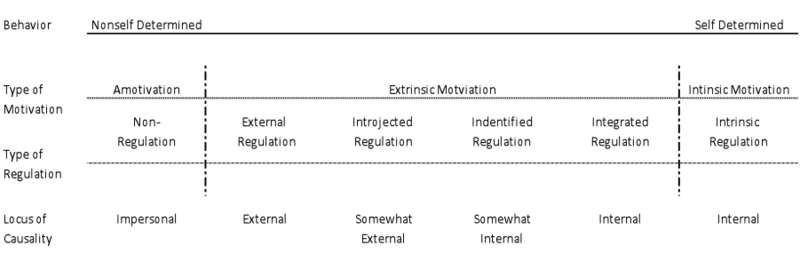
\includegraphics[width=0.8\textwidth]{Figures/oit.png}
    \rule{35em}{0.5pt}
  \caption{Organismic integration theory~\citep{ryan2000intrinsic}.}
  \label{figure:oit}
\end{figure}

SDT has been used to understand motivation for various activities or behaviours such as gaming~\citep{ryan2006:motivationalpull}, physical activity~\citep{power2011:obesity}, tobacco cessation~\citep{williams2006:testing} and energy saving~\citep{webb2013:self}. This study brings the motivational pull of gamification under the lens of SDT in order to understand how gamification can be used effectively in encouraging intermediaries to assist their respective beneficiaries in the utilization of personal health informatics. In the next section, the discussion of SDT is expanded through the lens of gamification.
\section{Self-Determination Theory Support in Gamification}
In order to understand why gamification may be important in intrinsic motivation, one has to understand the motivational triggers behind games.~\cite{knaving2013designing} framed the concept of games in terms of play and fun, where they conceptualized the terms as follows: (1) \emph{fun} is a rewarding and developmentally appropriate process necessary for survival, as it imparts humans with skills, knowledge and social cohesiveness; (2) \emph{play} is a voluntary engagement in an activity in order to have fun and feel pleasure; and (3) \emph{games} is formal play that is bound by rules. 

Games have defined goals and immediate feedback on progress towards those goals, and these are important mediators of optimal experience in play~\citep{knaving2013designing}.~One online survey~\citep{vella2013positively} with N=429 found that social play, relatedness during game play and flow (connection between goal setting and feedback) were some of the factors positively associated with players' psychological well-being.~\cite{ryan2006:motivationalpull} used self-determination theory to study motivational triggers in video games, where it was found that when aforementioned basic psychological needs were met, predicted the increase in enjoyment and the possibility of continuing to play the game in future. The importance of providing support for the three basic psychological needs has been emphasized  by situating the needs as part of motivational affordances to use ICTs with the objective of fostering motivation to use ICT systems~\citep{zhang2008motivational}. 

\cite{nakajima2013designing} argue that we should design systems to mimic the techniques used in games, to build emotionally engaging persuasive systems. The motivational aspects of gaming have steered researchers to explore their usage beyond the gaming context, and this has resulted in the advent of phenomena such as serious games and gamification. ~\cite{deterding2011game} considers gamification to involve borrowing ideas for motivating game design elements/patterns and applying them in a context outside the gaming environment. Gamification has a tendency to evoke intrinsic motivational experiences in users through gameful affordances~\citep{hamari2014persuasive}. Gamification is used outside the game context to increase interest in uninteresting but instrumental activities (e.g. physical activity and crowd-sourcing tasks such as image annotation). A systematic review on peer-reviewed studies found that the use of gamification was likely to have positive effects that are highly dependent on both the users of a gamified system and the context where a gamified system is used~\citep{hamari2014does}. Extrinsic integrated games have a practical advantage of having patterns that may scale well to different domains, while for intrinsically integrated games scalability may be a problem, and in practice it is much harder to design an intrinsically integrated game for each domain~\citep{preist2015use}.

\cite{hamari2014does} listed the most popular extrinsic motivators in gamification as ``\emph{points, leaderboards, story theme, badges, levels, goals, feedback, virtual rewards, progress and challenges}''. There are different schools of thought on whether gamification itself is a game or not. Most debates are centred around what a typical game entails (e.g. presence of rules, meta-games, immersion and voluntarism in their adoption)~\citep{seaborn2015:gamification}. According to~\cite{deterding2011game}, users of gamification can socially construct the meaning for what they consider gamification to be: they can perceive it as a game or, as some  other form of engagement depending on their context. The paper further argues that gamification is a gameful experience where an end user undergoes through an ``experiential flicker'' between different modes of engagement: gameful experience, playful experience or instrumental experience. This means that users alternate between perceiving a gamified tool as a game, and a state where a gamified system is perceived as instrumental for achieving a certain objective not related to game play. For instance, while users use a specific tool to achieve something, there is a possibility of the same people experiencing enjoyment from gameful or playful experiences.~\cite{seaborn2015:gamification} argued that the goal of gamified systems is different from games; therefore, it should rather be considered an act of integrating user experience with an activity outside the game context.~\cite{knaving2013designing} emphasized that while using gamification, the main activity being promoted should remain salient without being overshadowed by gamification; they recommended that designers should strike a balance between the preservation of an activity being promoted through gamification, and designing for playfulness. The goal of gamification should be to impart knowledge about the main activity being promoted, hence a design strategy should support both play and internalization.

\cite{sailer2013:psychological} provided examples of how game design elements can be mapped to the needs of competence, relatedness and autonomy; for instance, badges can be used to foster a sense of competence, while a leaderboard can be used to foster a sense of relatedness, as members of different teams are able to participate in competition with each other. A study by~\cite{hamari2013social} found the success of gamification to be dependent on social factors such as social influence, recognition, reciprocal benefit and network exposure, so in a gamified intervention, it is important to have a group of users that are committed to what a gamified system promotes.

\cite{mekler2013points} conducted a study to evaluate whether gamification harms intrinsic motivation. Gamification was added to crowd image annotation tasks. In that study it was found that gamification can increase engagement, but intrinsic motivation didn't change and was no different to the control group. Depending on how a gamified system has been designed, it can either foster or hinder the internalization of regulation that is externally rewarded. One way to foster intrinsic motivation is to ensure that gamification provides an optimal internalization (identified or integrated regulation).

There are some suggestions of how one could use gamification to promote motivation towards optimal internalization. An example is to make gamification meaningful. An experiment that examined facilitating contextual factors that can foster internalizing the regulation of a behaviour, found that factors such as framing the task with a meaning (providing a meaningful rationale), being sympathetic towards the behaver's  feelings and conveying choice fostered integrated regulation~\citep{deci1994facilitating}.~\cite{nicholson2012user} presented a framework for meaningful gamification that put the user at the centre. The framework was inspired by organismic integration theory explained above, situational relevance and situated motivational affordance, universal design for learning, and player-generated content. An example of meaningful gamification is where users are convinced that what they are doing is not just for the sake of playing a game but rather for contributing to a good cause. For instance,~\cite{mekler2013points} used points and a leaderboard to encourage participants in image annotation tasks and found that even though gamification did not harm intrinsic motivation, it negatively affected the quality of image annotation as participants were focusing on completing more tasks in order to advance in gamification. The same experiment was repeated, except this time it included gamification with meaningful framing, where participants were informed how each tagging was instrumental in improving computerized affective image categorization and, as a result, contributing towards an advancement in science. This was an appealing cause to the participants, hence it resulted in better quality tags being produced by participants in the meaningful framing condition~\citep{mekler2013disassembling} compared to participants in gamification without meaningful framing. In the context of this research, I hypothesized that pairing an intermediary and beneficiary that have a good social relationship would help intermediaries view the activity of assisting their beneficiaries as a good cause as they would be helping people they care about; hence it was anticipated that this framing would cause the collaborative gamified system to be perceived as meaningful.

The next section presents utilization of games and gamification in health interventions and what is lacking in literature as far as those interventions are concerned, with regard to supporting the utilization of personal health informatics through intermediary users.

\section{Utilization of Games in Personal Health Interventions}
Following the success of games as platforms for entertainment purposes, there is a paradigm shift towards using such platforms to influence positive changes in health behaviours~\citep{king2013gamification}. There is an increasing interest in using games to engage people with personalized health interventions~\citep{mccallum2012gamification}. Traditional design of games encourages people to remain sedentary; however, the new direction of research brings body movements into the game play. Games for health include but are not limited to exergames, games with purpose (serious games) and gamification. These classes of games are discussed in the next subsections. 
\subsection{Exergames}
Exergames combine exertion (body movements that are beyond sedentary activities) and video games. Exergames may include strength training, balance and flexibility activities~\citep{oh2010defining}. Exergames increase the amount of energy expended by the body~\citep{graves2010physiological}. Examples of exergames include  dance video games, e.g. Dance Dance Revolution~\citep{lieberman2006dance}, or games such as Nintendo Wii Fit~\citep{gobel2010serious}. There are also exergames that have been designed to be used for outdoor activities.~For instance, Zombies Run! is an outdoor exergame that gives users the experience of immersion while jogging; this immersion is achieved through interesting narratives about zombies who appear to chase the runner at specific points of the story. This makes the runner respond by running much faster in order to avoid being caught by zombies~\citep{southerton2013zombies}. With an exergame, one can become more active, but its use should never be confused with exercise~\citep{oh2010defining}. According to~\cite{caspersen1985physical} cited by~\cite{oh2010defining}, ``\emph{Exercise is doing a physical activity intentionally to improve or maintain physical fitness with a planned, repetitive, and structured format}''. Playing an exergame entails exertion, but it remains a physical activity which may be for entertainment purposes, unless that activity is performed according to the definition of exercise~\citep{oh2010defining}. However, playing an exergame is better than playing a sedentary video game, as the former promotes physical activity which is important in increasing energy expenditure. This form of energy expenditure, which doesn't fit into a category of exercise, is known as \emph{NEAT} -- non-exercise activity thermogenesis. NEAT activities such as walking, taking stairs or exergaming (playing exergames) have been found to expend a significant amount of energy~\citep{fujiki2008neat}. Exergames have application in health settings as they can be used to support rehabilitation~\citep{mccallum2012gamification}. In one study, the use of exergames was compared with traditional methods of physiotherapy. It was found that exergames performed significantly higher in scores of autonomy, presence, and in functional reach tests~\citep{smeddinck2015exergames}. The exergames consisted of a collection of different games that allowed players to perform bodily movements such as raising their hands in order to pick apples from a garden, and placing them in a basket near the ground. This required players to bend their bodies. Users had sensors attached to their bodies, and their bodily movements could make virtual avatars perform certain tasks on a screen. This is a common way of controlling characters in many games, including the sedentary ones which entail the use of physical input devices such as game consoles, keyboards, or other sensory mechanisms to support players' embodiment of virtual characters or avatars~\citep{berkovsky2012physical}. So the approaches used to control avatars in games for health purposes are somehow similar to the ones used in conventional electronic games. 

The benefits of exergames are not limited to younger populations.~\cite{brox2011exergames} revealed that exergames could also be accepted by elderly populations. In one study by~\cite{brauner2013increase}, an exergame was developed where players had to pick fruit and vegetables from a virtual garden using an avatar that represented them on screen. Interaction with an avatar happened through a Microsoft kinetic sensor for detecting body movements and gestures. The game was found to be enjoyable by the elderly participants. However, features to support personalization and persistent storage of players' information were not present in that game; in such a scenario players cannot resume from a previous state of the game play. In addition, the only interaction was through bodily movements. There was no complex navigation (in many other systems, several layers of user interfaces are required in order to reach the main feature). This implies that navigation to the main gaming interface was less sophisticated, and may have required less cognitive effort on the part of users in comparison to typical gamified personal health informatics systems, which may require users to navigate across several layers of user interfaces before firing an action. It is possible for a user interface of a personalized system to appear sophisticated to users who are not conversant in technology. Older adults are an example of a demographic group that might face barriers in navigating user interfaces.~\cite{chen2016social} evaluated an app that implemented social incentives to encourage obese and diabetic patients to exercise, and it was found that technical literacy is a challenge for older patients. A review on popular personal apps has revealed that many do not accommodate the needs of older adults~\citep{silva2014:smartphones}; hence this study emphasizes that one can leverage existing usage through intermediaries for such population groups, as this mode of interaction is already prevalent in many low-income communities of developing countries. Such an interaction may be possible in collectivist societies~\citep{parikh2006}. The idea of collectivism in the utilization of personal health systems has been emphasized in the dimension of having a community of users that collaborate in the management of health information~\citep{colineau2011motivating,grimes2009toward}, or different users of personal systems sharing health information among one another across social media~\citep{ploderer2014social}, but not in the respect of having one user supporting another user in their information needs through a single collaborative user interface. For instance, literature reports on exergames and systems that support competition in health self-reflection, where such systems involve  parents and children working together~\citep{grimes2009toward,saksono2015spaceship}, but their study was not done in the context of one user supporting the other user to navigate through user interfaces.
\subsection{Serious Games in Health}
Serious games have been defined as games that are designed to achieve a specific goal of change in the player's knowledge, attitude, physical ability, cognitive ability, etc. Serious games are sometimes referred to as games with purpose: their intention is to provide experience and emotion with the goal of conveying a meaning~\citep{marsh2011serious}. Areas in which serious games can be utilized for personal health include preventive (exergames), therapeutic (rehabitainment), assessment (self-ranking), educational (medical information) and informatics (personal health records)~\citep{mccallum2012gamification}. As serious games add user experience to an outside activity (probably an uninteresting one), there is an overlap of goals between serious games and gamification. The two terms are sometimes used synonymously (interchangeably).

There has been a rapid increase in the number of gamification-related studies in the persuasive technology field~\citep{hamari2014persuasive}. One prevalent utilization of gamification is to promote physical activity, with the aim of promoting NEAT physical activities as they are more omnipresent in people's daily lives compared with volitional sporting activities, which are mostly constrained by location and time~\citep{fujiki2008neat}. The urgent need to promote non-exercise physical activity is a result of the prevalence of electronic screens such as televisions and computers, which has increased the tendency of people to be more sedentary~\citep{berkovsky2010physical}. One study~\citep{levine2006non} cited in~\cite{fujiki2008neat} found that obese participants were spending more time (164 minutes longer on average) seated  compared with lean participants. There is a need for pervasive and ubiquitous computing to support people to become more aware of their lifestyle in order to foster an increase in non-exercise energy expenditure and reduce the quantity of calories consumed. This section provides examples of systems that use games/gamification in motivating particular healthy  behaviours through self-monitoring. These systems utilize various techniques such as points, avatars, virtual pets and leaderboards that have already been discussed above. 

\cite{lin2006:fish} developed and evaluated the Fish'n'Steps system, a computer game in which growth of a fish in a tank, together with its emotional state, is directly linked to footsteps of a player that have accumulated throughout the day. The application was evaluated with a total of 19 participants in a 14-week study. The findings indicated that the game catalysed the promotion of exercise and improvement of players’ attitudes towards physical activity. The authors observed that players' enthusiasm in playing the game had declined towards the end of the second week of using the application, mainly due to players already becoming accustomed to the new routines of a healthier lifestyle. 
  
\emph{{NEAT-o-Games}}~\citep{fujiki2008neat}, a comprehensive collection of PDA-based games, allows players to accumulate physical activity points which they can use in a virtual race. In order for an individual to accumulate points from physical activity, there is a wireless transmission of physical activity from a wearable accelerometer to a PDA, resulting in the player's animated avatar moving forward in a virtual race. Each player's position in the race corresponds to their current physical activity points. A player with the highest physical activity points leads the race. A player can also decide to use physical activity points to get hints while playing a puzzle-solving game called Sudoku. Using points in Sudoku means a player drops behind in a race game, and more steps (physical activity points) are required. In a pilot experiment with 8 participants, the authors indicated that participants increased their physical activity while enjoying playing the collection of games. 

The~\emph{Flowie} system, designed for home settings, is a virtual coach used to motivate elderly individuals to increase their amount of walking. The system consists of a frame casing with a touchscreen display that shows a flower whose vitality corresponds to the amount of physical activity captured by using context-aware sensors~\citep{albaina2009flowie}. A concept similar to the Flowie system is that of UbiFit Garden, which generates a garden with flowers of different types that discern different types of activity such as cardio, walking and housework~\citep{klasnja2009:using}. The authors showed the usefulness of living metaphors such as garden flowers in communicating information about physical activity level, as it makes an interaction experience to be more enjoyable and engaging to end users.

\emph{StepCity}, a strategy-based game~\citep{walsh2014stepcity}, is controlled through accumulated footsteps. In a StepCity game, players connect their Fitbit accounts\footnote{https://www.fitbit.com/} to the game. Players' accumulated steps can be used as currency in the game to buy buildings to place in players' respective cities that produce gold and increase population. Buildings have side effects, as cheaper buildings produce more crime while more expensive ones produce none. Players can move through various stages of civilization, and a leaderboard is used to rank cities by the amount of gold, crime and population. In evaluation there were three experimental conditions: the control group (only Fitbit), the social interaction experience (app supporting interaction between participants), and the StepCity game. The results of evaluating the game with 50 users showed that newer Fitbit users (n=41) had more steps than the amount accumulated during the control period (at the beginning, before starting to use the game) without statistical significance; however, the overall results were inconclusive.  

There are also other studies that used gamification to motivate adolescents or teenagers in behaviours such as frequent monitoring of blood glucose or physical activity~\citep{arteaga2010:persuasive,cafazzo2012:bant}. Apart from interventions that target promotion of physical activity, there are game-based apps designed to encourage healthy eating. An example of such an app is a mobile game called \emph{It's Time to Eat}, which was specifically designed to motivate children to practise healthy eating habits through taking care of their virtual pets~\citep{pollak2010s}. In the game, players select a pet from a range of options such as a worm, dinosaur, dog and tree. Then players are required to take care of their selected pets. The first step is for players to choose names for their pets. The process of selecting a pet and naming it is meant to give a player a sense of control or autonomy. Caring for a pet entails a player feeding it by uploading a photo of their breakfast, and then a nutritionist gives it a certain score. Based on the total score, a virtual pet responds with an emotional state. A healthy breakfast results in a pet becoming happy, while an unhealthy meal makes the pet sad. The finding from this study indicated that kids who had played the game had an inclination towards eating a healthy breakfast more frequently than those who didn't play the game~\citep{pollak2010s}. Another diet-based game is called \emph{LunchTime}~\citep{orji2013lunchtime}, aimed at educating people to make healthy choices while eating away from home. This application utilizes the following persuasive strategies: goal setting, feedback, social influence and rewarding mechanisms. In~\cite{orji2013lunchtime}'s study, the game was played by a group of friends visiting a restaurant as customers. The game awarded points to players according to how healthy the choices of their meals were. A 10-day evaluation  of LunchTime, with 6 participants (three males and three females) aged between 19 and 40 years of age, indicated that the application facilitated learning and reflection. In addition to that, attitudes towards healthy eating showed improvement at the endline in comparison to the baseline. 

An example  of a different use of games is the supporting of heart-rate monitoring, for instance in the case of \emph{Live Pulse Games}~\citep{han2014designing,han2015balancing}. Live Pulse Games is a collection of games that employ a novel technique to measure users' heart rate in real time, by having them play casual games on their mobile phones. In order to gain some in-game control, the player has do some covering of the camera lens with their fingertips during the game play. For instance, one game within Live Pulse Games is called \emph{City Defender}. In this game, an end user has to load the anti-aircraft artillery through lens-covering actions. The heart rate is computed by detecting changes  in  blood transparency in the user's fingertips.
 
Another approach to gamification does not involve adding user experience to a targeted health behaviour; instead, a motivating sedentary game is interlaced with the targeted health behaviour. This approach is based on Premack's principle~\citep{premack1959toward}, which suggests using an event with high probability, such as playing a computer game, to motivate an activity with low probability, such as doing physical activity. An example of a game that utilizes such an approach is one called \emph{PLAY MATE}~\citep{berkovsky2010physical,berkovsky2012physical}. This game takes advantage of motivation factors in video games by introducing a burst of physical activity during a session of  sedentary game play. \emph{PLAY MATE} is an alteration of an open-source computer-based game called \emph{Neverball}, which gives a player a limited amount of time to collect coins~\citep{berkovsky2012physical}. In the design of PLAY MATE, incentives of extra time are given to a player for each jump that is performed in the middle of a session of sedentary game play~\citep{berkovsky2012physical}. Jumps are detected through a sensory device (built with an accelerometer and gyroscope) worn on the waist. The preliminary evaluation of this system indicated that skilled players had a tendency to perform fewer jumps compared with less skilled players; hence the game was modified to include an adaptive algorithm by which the level of difficult was personalized according to a player's completion time of previous levels.

A similar idea implicitly utilizes Premack's principle~\citep{premack1959toward} in education settings.~\cite{preist2015use} looked at enjoyable game playing combined with revising for an examination.Their approach used the F2P (free-to-play) game business model, where users are presented with a fully functioning game that is freely available but has an option to do micro-payments in order to either speed up game play (e.g. speed up resource gathering used to advance technology for combat in a strategy game) or provide access to virtual goods. This study used a game strategy similar to Clash of the Clans to motivate 15- to 16-year-old children to revise in preparation for a mathematics examination. The option of micro-payment was substituted with virtual currency earned through taking revision tests at any time within the game play. An experiment was performed to discern the effectiveness of the educational game in comparison to two groups which were control, and the quiz generator software. The findings from that study indicated a statistically significant improvement in performance (based on pre-post scores of the test) on learners that were assigned to the game group~\citep{preist2015use}. Even though the experiment was conducted in the learning context, one could adapt the same concept to the context of promotion of health behaviours.

Most of the health-based interventions reported in the literature are carried out in contexts that are not constrained by resources, with the exception of a few, such as the one that developed an exergame for families in low socio economic areas~\citep{saksono2015spaceship}, or another study that used user-centred approaches in the development of mobile game-based applications for the promotion of physical activity in youths with low socioeconomic status~\citep{blackman2016developing}. Literature on utilization of serious games in developing world contexts is scarce and existing studies tend to focus on education~\citep{kam2008designing,botha2015icts}.

In this research, the focus was on health interventions within the context of low-resource settings of a developing country, which may not be the same as a context of low socioeconomic status in developed countries. One of the drawbacks of those gamified personalized interventions is that they tend to be designed for direct/primary users of technology, as only direct beneficiaries are considered; leaving out indirect beneficiaries (those that depend on intermediary users for facilitating access to user interfaces). In most of these interventions, the person (an adult or young person) who is a targeted beneficiary of the information on the app is expected to be an actual manipulator of the user interfaces of such a system. Most of the motivational incentives provided by such systems target direct users, who in most cases are younger and technologically literate. None of the aforementioned studies have explored the utilization of gamification where one user facilitates an interaction process while an actual beneficiary remains an observer or indirect/secondary user. Thus this study aimed to explore how one could implement motivational incentives (affordances) to target a pair that consists of an intermediary user and a beneficiary user. Literature on intermediated technology use has shown that young people within a community may fit well as intermediary users. In addition, young people have more of an inclination to play computer games than the elderly~\citep{brauner2013increase}. There is an opportunity for leveraging the  motivation of young people through gamification to foster collaboration between adults and children, with the goal of children engaging adults who may be less conversant or less motivated to engage with gamified personal health informatics. 

\begin{flushright}
\end{flushright}
